% Chapter Template

\chapter{Fluorescence Microscopy} % Main chapter title

\label{chap:Chapter2} % Change 2 to a consecutive number; for referencing this chapter elsewhere, use \ref{chap:Chapter2}
%\citep{Biehlmaier2013}
%\citep{Svoboda2007}
%\citep{Svoboda2009}
%\citep{GonzalezWoods2002}
%\citep{Pratt2001}
%\citep{Soile2004}
%\citep{Matula2006}
%\citep{Rohr2010}
%\citep{Matula2000}
%\citep{Kozubek2001}
%\citep{Petran1985}
\textcolor{red}{What is fluorescence microscopy? What's it's purpose in the thesis?	Photoluminescence -> fluorescence and phosphorescence. Discovery of fluorescence: Brief history and evolution. Brief discussion on the remainder of the chapter.}
Fluorescence microscopy has become an essential tool in diverse fields, such as petrology, semiconductors, etc, and has especially been established as a choice imaging technique in cellular and molecular biology for visualisation of cells and tissues \citep{Spring2003,Danek2012,Hubeny2008,Fatima2008,Matula2012}.
In this thesis we confine our attention to its use in cellular biology.

Certain substances emit radiation when irradiated with a higher intensity light, such as ultraviolet (UV), blue or green, which is off a longer wavelength than that of the exciting light, this is known as \textit{Stokes' Law}.
This phenomenon is known as \textit{photoluminescence} \citep{Koch1972,Vaughan2015,Sarder2006,AbramowitzDavidson2016}.
There are two types of photoluminescence. If emission persists at an appreciable level after the exciting light is turned off, then we call this \textit{phosphorescence}.
If emission persist only so long as the exciting light is on, then we call this \textit{fluorescence} \citep{Koch1972,SpringDavisdson2016}.

The first observance and publishing of fluorescence is credited to Sir John Frederick William Herschel around 1852.
In 1852, Sir John George Stokes published a 100 page treatise about this luminescent phenomenon and coined the term \textit{fluorescence}, over Herschel's \textit{dispersive reflection}, when he observed that the mineral \textit{fluorite} emitted red light when irradiated by ultraviolet (UV) light \citep{Dobrucki2013,Danek2012}.

In the remainder of this chapter we present the underlying principles of fluorescence, how specimens are fluorescently marked, the optical principles of microscope design, image acquisition, image processing and common analysis in cellular biology.
We only go so far in depth as to present a rudimentary understanding of fluorescence microscopy as is necessary for the comprehension of this thesis.

%----------------------------------------------------------------------------------------
%	SECTION 1
%----------------------------------------------------------------------------------------

\section{Physics of Fluorescence}
\label{sec:PhysicsOfFluorescence}

\textcolor{red}{Why is it necessary to understand the principles of fluroescence? Simple description of the fluorescence process. A more in-depth explanation of the fluorescence process and why stuff goes wrong  e.g. phosphorescence, fading, etc.}
Fluorescence microscopy is a cross-disciplinary field.
It is encouraged, if not necessary, to have a photophysical understanding of the principles of fluorescence, for biologists and computer scientists.
The knowledge of the "under the hood" mechanics of fluorescence empower computer scientists to make informed and directed research in terms of image processing.
The aim here is to present an elementary introduction into the physics of fluorescence.

\begin{figure}[!t]
	\centering
	\subfigure[]
	{
		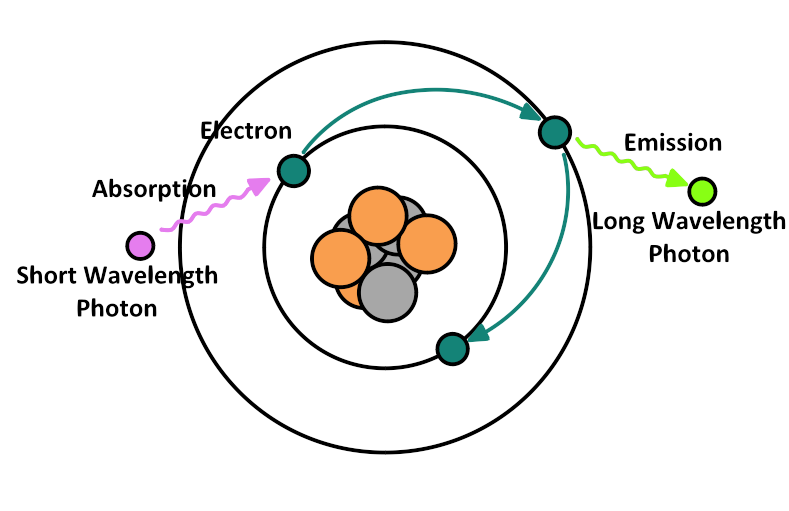
\includegraphics[width=0.4\columnwidth]{molecular_absorption.png}
		\label{fig:molecularabsorption}
	}
	\subfigure[]
	{
		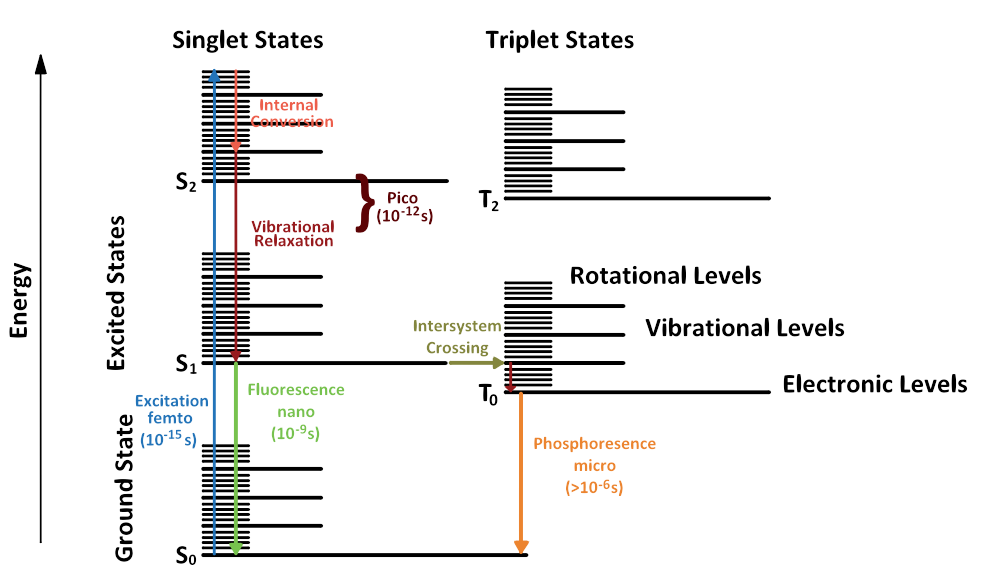
\includegraphics[width=0.56\columnwidth]{jablonski_diagram.png}
		\label{fig:jablonski}
	}
	\caption{\textbf{(a)} Simplified fluorescence process. \textbf{(b)} The Jab{\l}o{\'n}ski diagram depicting the electronics states from photon absorption to photo emission.}
	\label{fig:fluorescence_electron_states}
\end{figure}

The overall principle of fluorescence can be explained in three steps \citep{Nobel2016} as illustrated in \autoref{fig:molecularabsorption}: 
(1) Energy is absorbed by an atom upon collision with a photon.
(2) The atom becomes excited and an electron jumps to a higher energy level.
(3) Shortly after jumping to the higher energy level the electron returns to the ground state and emits a photon.

\begin{definition}[Excitation and emission]
	One of the best ways to visualise the fluorescing process is using a Jab{\l}o{\'n}ski diagram.
	A detailed Jab{\l}o{\'n}ski diagram is shown in \autoref{fig:jablonski}. 
	When a photon collides with an atom, all its energy is transferred to the atom. The energy of the photon is inversely related to it's wavelength, $E = h \frac{c}{\lambda}$, where $h$ is Planck's constant and $c$ and $\lambda$ are the speed and wavelength of light in a vacuum respectively.
	This increase in energy moves an electron from the ground state $S_0$ to a higher level energy state.
	Depending on the energy of the photon and the number of photons absorbed by the photon the electron can move to different energy levels e.g. $S_1, S_2, etc$.
	This process happens almost immediately in the order of femtoseconds($10^{-15}s$).
	Before moving to the lowest next higher energy level ($S_1$), some energy is lost due to internal conversion and vibrational relaxation.
	When the electron spontaneously decays from $S_1$ to $S_0$ it emits a photon of longer wavelength than the absorption photon.
	This happens few nanoseconds ($10^{-9}s$) after excitation.
	
	The difference in wavelength of the emission photon and excitation photon is known as the \textit{Stokes' Shift} or \textit{Stokes' Law}.
	The larger the Stokes' Shift the easier it is to separate the emission light from the excitation light \citep{Spring2003}.
	The emission curve is often a mirror image and shifted to longer wavelengths than the excitation curve as illustrated in \autoref{fig:excitationandemissionspectra}.
\end{definition}

\begin{definition}[Fluorophores]
	Substances that exhibit the fluorescent property are called fluorophores, also known as \textit{fluorochromes} or \textit{fluoresent dyes}.
	Early investigations showed that many substance naturally posess fluorescent properties, such as minerals, crystals, resins, crude drugs, butter, chlorophyll, vitamins, etc \citep{Spring2003}.
	This is known as \textit{autofluorescence}.
	Substances that do not fluoresce must be \textit{stained} such that it can be observed through a fluorescent microscope, more on this later.
\end{definition}

%\begin{definition}[Jab{\l}o{\'n}ski diagrams]
%	Stuff for this section.
%\end{definition}

%\begin{definition}[Excitation spectra]
%	Stuff for this section. Electronic States
%\end{definition}

%\begin{definition}[Emission spectra]
%	Stuff for this section. Electronic States
%\end{definition}

\begin{definition}[Intersystem crossing]
	If the electron spin as the electron transfer between energy states is preserved then the energy states are known as \textit{singlet states}. It is also possible for the electron to reverse it's spin. This is very unlikely and is known as \textit{forbidden transition} in Quantum mechanics. When this happens the electron is said to be in a \textit{triplet state}, see \autoref{fig:jablonski}. The only way for the electron to reach the ground state is to again undergo another forbidden transition which is unlikely. When this does eventually happen the electron may emit a photon and this phenomenon is known as \textit{phosphorescence}. This process takes much longer, in the order of microseconds ($10^{-6}s$).
\end{definition}

%\begin{definition}[Quantum yield]
%	Stuff for this section. Electronic States
%\end{definition}

\begin{figure}[!t]
	\centering
	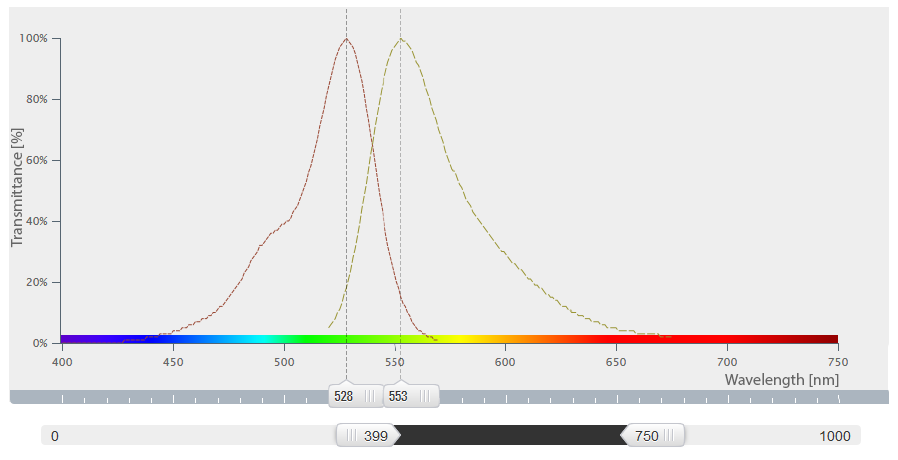
\includegraphics[width=\columnwidth]{Fluor532_ExcitationEmissionSpectrum.png}
	\caption{Normalised Excitation and Emmision Spectra of the Alexa Fluor 532 flurophore. The emmission maximum is at $553nm$ which is a more yellow-green than excitation maximum at $528nm$. This image was generated using FluoScout\texttrademark\, web application by Leica Microsystems for determining the optimal fluorescence filter cube set. %\url{http://www.leica-microsystems.com/fluoscout/}
	}
	\addloflink{http://www.leica-microsystems.com/fluoscout/}
	\label{fig:excitationandemissionspectra}
\end{figure}

%----------------------------------------------------------------------------------------
%	SECTION 2
%----------------------------------------------------------------------------------------

\section{Specimen Labelling}
\label{sec:SpecimenLabelling}

\textcolor{red}{Why do specimens have to be stained? What is is staining?}
Many of the components of interest, such as cell nuclei, cytoplasm, genes, chrosomes, proteins, do not possess a high degree of, if not any,  autofluorescence. 
In this scenario, these components can be marked with a fluorescent dye \citep{Tsien1998}, also known as a fluorophore or fluorochrome, a substance that can bind to a specific target whose excitation and emission spectra are well known. 
This is known as staining \citep{Danek2012,Hubeny2008,Dobrucki2013}. 
Once the specimen is stained it can be indirectly observed using a fluorescence microscope.

\textcolor{red}{What are the most common staining protocols?}
The most prevalent staining techniques are fluorescence in-situ hybridisation (FISH) and immunostaining \citep{Danek2012,Fatima2008,Kozubek2001_2,Theodosiou2007}.

\begin{definition}[FISH staining]
	\textcolor{red}{What is FISH?	What is the FISH staining techniques used for?}
	FISH is a molecular cytogenetic technique that uses flourophores that bind to selected regions in nucleic acids \citep{Danek2012,Fatima2008}.
	FISH is the most frequently used staining technique used primarily for visualisation and localisation of nucleic acid sequences, chromosomes, cytplasm or organelles which contain those acids \citep{Hubeny2008}.
	This makes FISH highly attractive for finding specific features in DNA and RNA used in genetic diagnosis and research, medicine and species identification \citep{Amann2008,Fatima2008}.
	Figure \ref{fig:FISH} is a capture of mouse chromosomes using the FISH staining technique.
\end{definition}

\begin{definition}[Immunostaining]
	\textcolor{red}{What is Immunofluorescence and the two main types, what is the difference between the two, and which is more common? What is the Immunofluorescence staining techniques used for?}
	Immunofluorescence is the detection method where an antibody is used to detect an antigen in a tissue or a cell using fluorescence. Flourophores are usually conjugated onto antibodies, which are proteins that are designed bind to specific antigens, target proteins, on a cell \citep{CudeBurke2014}.
	The two types of immunofluorescent detection are immunocytofluorescence (ICF) and immunohystofluorescence (IHF).
	It must not be confused with immunocytochemistry (ICC) and immunohistochemistry (IHC).
	\textit{Immuno} refers to the immunological technique, i.e. the binding of antibodies to antigens.
	\textit{Cyto} refers to cells, i.e. cells without the extracellular membrane.
	\textit{Histo} refers to tissue i.e. cells with the extracellular membrane.
	\textit{Chemistry} refers to the chemical method of detection, e.g. a change in colour.
	\textit{Fluorescence} detection by emission of light \citep{Katikireddy2011}.
	Figure \ref{fig:IHC} shows the detection of the p53 Binding Protein 1 in perfusion fixed frozen sections of rat kidney.
\end{definition}

\begin{definition}[Live-cell staining]
	\textcolor{red}{FISH and IHC cannot stain live cells. Why? How can we stain live cells?}
	The previously discussed staining techniques are not suitable to observe living cells.
	The fluorescent dyes used are phototoxic and cause cells to die. The circumvent this problem an elegant solution has been devised.
	Instead of staining, the cells are modified to produce a fluorescent substance in the target structures.
	Derivatives of the \textit{green fluorescent protein} (GFP), isolated from the \textit{Aequorea victoria} jellyfish \citep{Tsien1998,LichtmanConchello2005,Fatima2008}, are used as it generates a strong photon emission and is non-toxic to living cells \citep{Danek2012,Hubeny2008,Dobrucki2013}.
\end{definition}

\textcolor{red}{Important notes about fluorophores and the impact on image quality?}

\begin{figure}[!t]
	\centering
	\subfigure[]
	{
		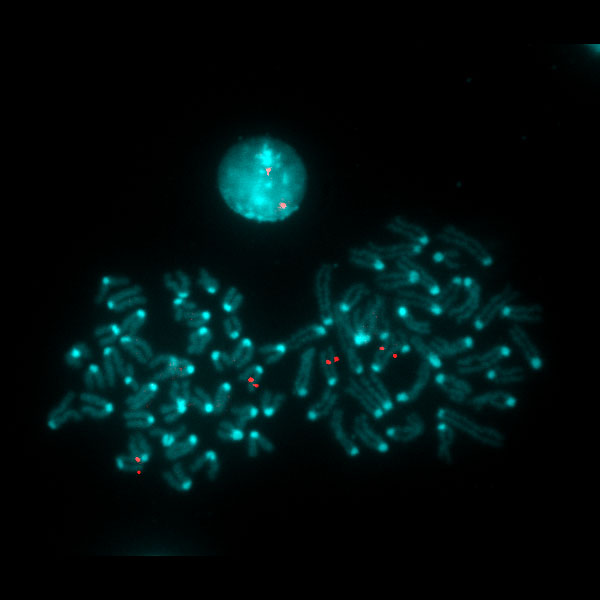
\includegraphics[width=0.495\columnwidth]{fish1.jpg}
		\label{fig:FISH}
	}
	\subfigure[]
	{
		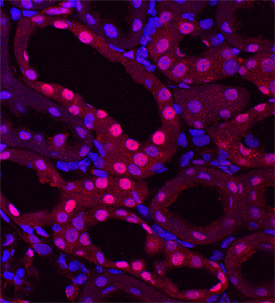
\includegraphics[width=0.45\columnwidth]{ihc1.jpg}
		\label{fig:IHC}
	}
	\caption{\textbf{(a)} FISH (Fluorescent 'in-situ' Hybridization) in mouse chromosomes using a BAC clone labeled with Spectrum Orange. The picture shows two metaphases and one interphase with two signals in each exampling a homozygous mouse for a transgenic clone. Image Source: "All About the Human Genome Project" Genetic and Genomic Image and Illustration Database. %\addloflink{https://unlockinglifescode.org/media/images/} %\url{https://unlockinglifescode.org/media/images/}. 
	\textbf{(b)} p53 Binding Protein 1 (53BP1) was detected in perfusion fixed frozen sections of rat kidney using Goat Anti-Human 53BP1 Antigen Affinity-purified Polyclonal Antibody (Catalog \# AF1877) at 15 $\mu$g/mL overnight at 4$^{\circ}$C. Tissue was stained using the NorthernLights\texttrademark 557-conjugated Anti-Goat IgG Secondary Antibody (red; Catalog \# NL001) and counterstained with DAPI (blue). Specific staining was localized to nuclei of epithelial cells in convoluted tubules. Image Source: R\&D Systems' IHC image database.}
	%\addloflink{https://www.rndsystems.com/resources/ihc-images/53bp1}}
	%\url{https://www.rndsystems.com/resources/ihc-images/53bp1}.}
	\addloflink{https://unlockinglifescode.org/media/images/}
	\addloflink{https://www.rndsystems.com/resources/ihc-images/53bp1}
	\label{fig:stainingtechniques}
\end{figure}

%----------------------------------------------------------------------------------------
%	SECTION 3
%----------------------------------------------------------------------------------------

\section{The Epifluorescence Microscope and Image Acquisition}
\label{sec:TheEpifluorescenceMicroscope}

\begin{figure}[!t]
	\centering
	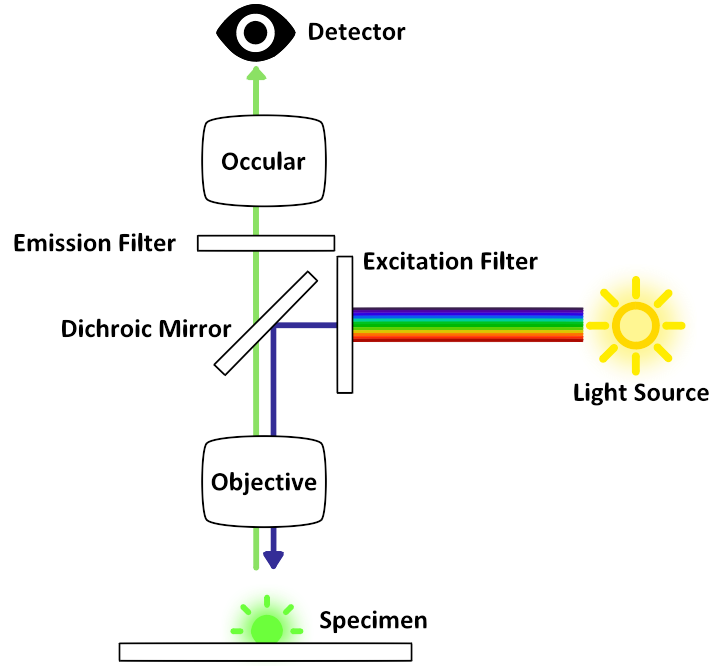
\includegraphics[width=0.4\columnwidth]{Epifluorescence_Microscope.png}
	\caption{The schematic of the epifluorescence microscope.}
	\label{fig:epifluorescencemicroscope}
\end{figure}

\textcolor{red}{What is a fluorescent microscope? Schematic layout of a fluorescence microscope? Function and purpose of each component in the fluorescent microscope?}
A fluorescence microscope is an optical microscope that is designed specifically to exploit the principle of fluorescence to allow for the observation of flourescently labelled specimens \citep{Hubeny2008,Sarder2006,Dobrucki2013,Andrews2002,Fatima2008}.
There are many types of fluorescent micrcoscopes avaialble but the favoured type among many biologists and geneticists is the epifluorescent microscope \citep{Rice2016,AbramowitzDavidson2016}.
The schematic of the epifluorescent micrcoscope is illustrated in \autoref{fig:epifluorescencemicroscope}.

\begin{definition}[Light source]
	\textcolor{red}{What sort of light needs to be generated? What sort of lamps are used? Advantages and disadvantages of certain lamps.}
	The light source is typically a high-luminance light source e.g. Mercury or Xenon arc lamps, LEDs, lasers, etc  \citep{Danek2012,Hubeny2008,Aswani2012,Rice2016,ThermoFisher2016}.
	The primary criterion for choosing a light sources is that its characeristic peaks must coincide with the excitation spectrum of the fluorophores being used \citep{LichtmanConchello2005,Spring2003,Fatima2008}.
	Wavelength coverage spans from near infra-red to UV. Mercury and Xenon arc lamps are expensive, an inexpensive and lightweight alternative is bright LEDs \citep{Fatima2008,Dobrucki2013,Aswani2012,Koch1972}.
\end{definition}

\begin{definition}[Excitation filter]
	\textcolor{red}{What is an excitation filter? Why is it needed?}
	The incoming light from the light source is typically mulispectral \citep{SpringDavisdson2016}. 
	The excitation filter is a wavelength selection filter which is placed in the path of the incoming light and filters through only those wavelengths in the absorption spectrum of the fluorescent dye \citep{ThermoFisher2016,Danek2012,Hubeny2008,LichtmanConchello2005,Spring2003,CudeBurke2014,Fatima2008,Dobrucki2013}.
\end{definition}

\begin{definition}[Dichroic mirror]
	\textcolor{red}{What is a dichroic mirror? Why is it needed?}
	Also known as a \textit{dichroic beam splitter}.
	This is placed at a 45$^{\circ}$ angle and reflects the short-wavelenght light filtered through the excitation filter at a 90$^{\circ}$ angle towards the specimen \citep{Danek2012,Hubeny2008,Spring2003,CudeBurke2014} and allows the long-wavelength light from the fluorescing specimen to pass through to the detector \citep{LichtmanConchello2005,Koch1972}, thus serving as a separation filter between the absorption and emission light \citep{Fatima2008,Dobrucki2013}.
\end{definition}

\begin{definition}[Objective]
	\textcolor{red}{What is the objective? Why is it needed?}
	The incoming light reflected of the dichroic mirror passes through the objective lens before reaching the specimen \citep{Danek2012,Hubeny2008,LichtmanConchello2005,Spring2003}.
	Emission light from the fluorescing specimen is gathered in the objective lens and passed through to the dichroic mirror.
\end{definition}

\begin{definition}[Specimen]
	\textcolor{red}{Say something about the specimen, for wholeness sake.}
	The specimen is irradiated by the incoming light from the objective and emits long-wavelength light in all directions.
	The specimen is stained with a flourophore whose absorption and emission curves are well known.
	This is important since the light source and the interference filters are chosen using the peaks of these curves.
\end{definition}

\begin{definition}[Emission filter]
	\textcolor{red}{What is an emission filter? Why is it needed?}
	Also known as a \textit{barrier filter} \citep{LichtmanConchello2005,Spring2003,Koch1972}.
	The light coming from the specimen contains multiple wavelengths and the dichroic mirror is used to filter out the shorter wavelength light.
	The emission filter is further  used to filter out the wavelengths that correspond to the emission wavelengths of the fluorophore \citep{CudeBurke2014,Danek2012,Hubeny2008,SpringDavisdson2016,ThermoFisher2016}.
\end{definition}

%\begin{definition}[Occular]
%	\textcolor{red}{What is the occular why is it needed?}
%	Purpose of the occular.
%\end{definition}

\begin{definition}[Detector]
	\textcolor{red}{What is the detector why is it needed?}
	The dector is used to capture the emission light and can further digital form the image.
	The detector is usually a photodector such as a CCD (charge-coupled device) camera or a photomultipler tube \citep{Danek2012,Hubeny2008,LichtmanConchello2005,Spring2003,Murphy2001}.
	It is vital that an appropriate detector be chosen as this has direct impact on image quality \citep{Fatima2008}.
\end{definition}

\textcolor{red}{Other Types of Fluorescence Microscopes: Confocal, TIRF. Acquisition: CCD, Hardware setup effect on image quality, Numerical Aperture, Sub-diffraction}
The type of fluorescence image data that needs to be captured is application dependant and this impacts the decision on which type of microscope to use.
The \textit{widefield}, or conventional, microscope produces 2D image data.
3D image data cannot be captured directly.
Instead, a series od 2D images are captured to form a 2D stack. The 3D image is then constructed in software.
In this scenario, the most common choice of micrscope is the \textit{confocal laser scanning microscope} (CLSM).
This microscope system is expensive and acquisition is slower.
An economical alternative is the \textit{confocal spinning disk miscroscope}.
To detect single molecules, the favoured technique is \textit{total internal reflection fluorescence} (TIRF) which can be achieved by a modification of the epifluorescence micrcoscope.

%----------------------------------------------------------------------------------------
%	SECTION 4
%----------------------------------------------------------------------------------------

\section{Image Processing}
\label{sec:ImageProcessing}

\textcolor{red}{Limitations in Fluorescence Imaging. Preprocessing: Point Spread Function deconvolution, etc. Segmentation }
Due to the physical nature of the fluorescence and image acquisition process, there are many factors that can degrade image quality.
There are measures that can be taken to largely mitigate some problems but they can never be completely abated.
The presence of these factors directly affect segmentation accuracy and subsequently higher level analysis.
Therefore, images are processed prior to segmentation to suppress the artefacts and reconstruct the original data \citep{Danek2012} or better yet enhance it.
\Cref{chap:Chapter7} takes a step in this vain.
Here we present some of the commonly occuring factors that reduce image quality and the methods used to mitigate them, and some of the techniques employed for segmentation.

\subsection{Preprocessing}
\textcolor{red}{Write a little something on preprocessing.}

\begin{definition}[Nonuniform illumination]
	\textcolor{red}{What causes uneven illumination? What techniques are done to reduce it's effect. Vignette effect, etc.}
	There are many factors that could contribute to nonuniform illumination.
	The specimen layer will not be uniformly lit if the  arc lamp is not properly focussed on the black aperture.
	To prevent this from happening, a liquid light guide-based light source, which provide even illumination may be used \citep{LichtmanConchello2005}.
	If the light brightness diminished towards the edges of the image then this is known as the \textit{Vignette effect}.
	Common techniques to suppress this distortion is \textit{background correction}, also known as \textit{flat-field correction}, \textit{background flattening} or \textit{shading correction} \citep{Danek2012,Fatima2008,Murphy2001}.
	Other causes of nonuniform illumination are inhomogenous detector sensitivity, autofluorescence, dirt particles in the optical system or nonspecific sample staining.
	An example of the Vignette effect is illustrated in \autoref{fig:Vignette}.
	Computational schemes to eliminate nonuniform illumination have been well researched, although recently it hasn't recived too much attention \citep{Young2001,Ghauharali1998,Model2001,Model2001_2}.
	
	\begin{figure}[!t]
		\centering
		\subfigure[]
		{
			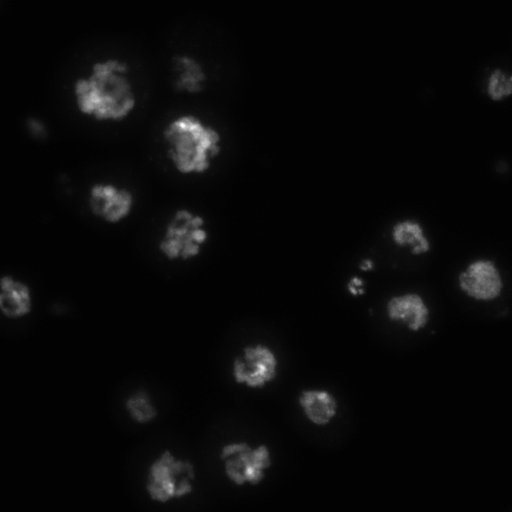
\includegraphics[width=0.31\columnwidth]{uneven_orig.jpg}
			\label{fig:ImageProcessingOriginal}
		}
		\subfigure[]
		{
			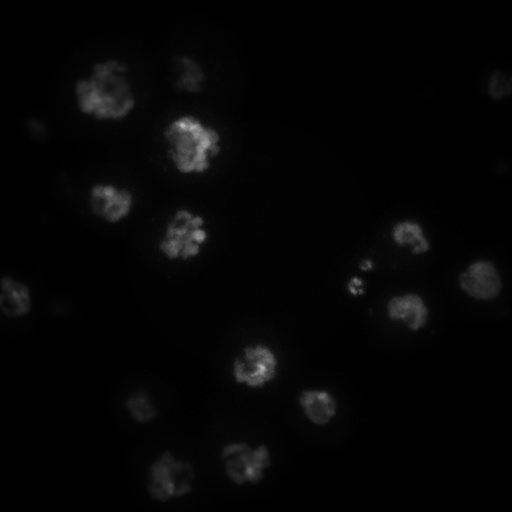
\includegraphics[width=0.31\columnwidth]{uneven.jpg}
			\label{fig:Vignette}
		}
		\subfigure[]
		{
			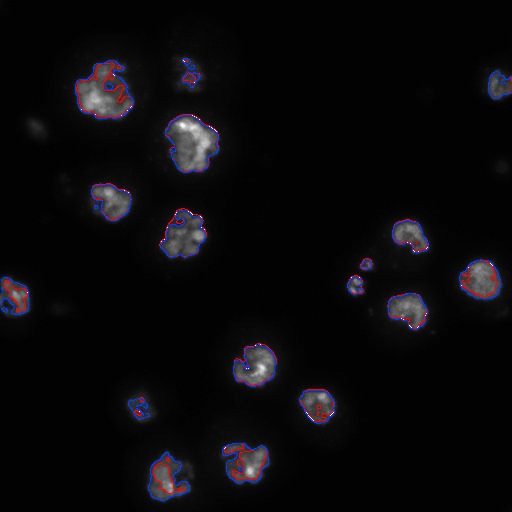
\includegraphics[width=0.31\columnwidth]{uneven_final.jpg}
			\label{fig:IlluminationSegmented}
		}
		\caption{The effect of nonuniform illumination on segmentation. \textbf{(a)} Original image. Image source: The Cell Image Library \citep{cil:21739}. \textbf{(b)} Nonuniformly illuminated image. The Vignette effect. \textbf{(c)} K-means clustering using the Euclidean distance metric and 2 clusters. The blue curve is from the original, the red curve is from the nonuniformly illuminated image. Notice that less of the object is recognised towards the edges.}
		\addloflink{http://www.cellimagelibrary.org/images/2173}
		\label{fig:illumination}
	\end{figure}
\end{definition}

\begin{definition}[Fading]
	\textcolor{red}{What causes quenching and bleaching? What techniques are done to reduce it's effect. Why is photobleaching worse?}
	The reduction of emission intensity is called \textit{fading}, of which there are two types: \textit{quenching} and \textit{bleaching}.
	
	Quenching is a reversible loss of fluorescence owing to a variety of nonradiative energy-loss mechanisms such as collisions with nearby acceptor molecules, a phenomenon known as \textit{resonance energy transfer}.
	This phenomenon is useful in studying molelcular interactions below the lateral resolution of the light microscope through a technique called \textit{fluorescence resonance energy transfer} (FRET) \cite{Spring2003,Danek2012,LichtmanConchello2005}.
	
	Bleaching refers to all processes that cause a fluorescent signal to fade permanently \citep{LichtmanConchello2005}.
	From the fluorescence process presented in \Cref{sec:PhysicsOfFluorescence}, one may assume that, under the proper conditions, a fluorochrome has the ability to fluoresce indefinitely.
	However, this is not the case. There is a limit number of cycles before permanent bleaching \citep{LichtmanConchello2005}.
	\Cref{fig:bleaching} illustrates the effect of photobleaching.
	\textit{Photobleaching} is the most prominent form of bleaching.
	It is due the interaction of the fluorophore with an oxygen molecule.
	This can move the oxygen molecule to an excited singlet state, which then becomes a reactive molecule.
	When in this state, the oxygen molecule can participate in many chemically destructive reaction with organic molecules causing \textit{phototoxicity} \citep{Danek2012}.
	Photobleaching is used to study diffusion and motion through a technique called \textit{fluorescence recovery after photobleaching} (FRAP) \citep{LichtmanConchello2005,AbramowitzDavidson2016}.
	
	Photobleaching cannot be avoided but it be can pushed back.
	The aim in the measures to avoid photobleaching is to take a longer time to reach \textit{reciprocity failure} \citep{AbramowitzDavidson2016}.
	This is done by shortening exposure times and using less intensive excitation light.
	This, however, yields low contrast images.
	These images with low signal-to-noise \citep{Murphy2001} ratio (SNR) are more difficult to segment hence contrast enhancement must be performed on the images prior to segmentation \citep{Boppart2005}.
	\begin{figure}[!t]
		\centering
		\subfigure[]
		{
			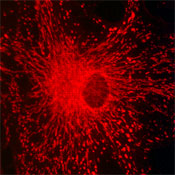
\includegraphics[width=0.31\columnwidth]{canvas.png}
			\label{fig:ImageProcessingOriginal2}
		}
		\subfigure[]
		{
			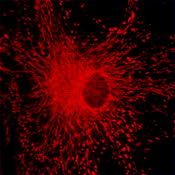
\includegraphics[width=0.31\columnwidth]{canvas10.png}
			\label{fig:Photobleach1}
		}
		\subfigure[]
		{
			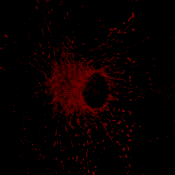
\includegraphics[width=0.31\columnwidth]{canvas20.png}
			\label{fig:Photobleach2}
		}
		\caption{The effect of photobleaching. Image Source: Molecular Expressions \citep{MolecularExpressionsPhotobleaching}. 
			\textbf{(a)} Original image at $t=0s$.
			\textbf{(b)} Image after $t=10s$.
			\textbf{(c)} Image after $t=20s$.
			}
		\label{fig:bleaching}
	\end{figure}
\end{definition}

\begin{definition}[Image distortion]
	\textcolor{red}{What causes image distortion (PSF)? What techniques are done to reduce it's effect.}
	The major contributing factors to image distortion are: The \textit{point spread function} (PSF) and noise \citep{Sarder2006}.
	Image formation can be approximated by 
	\begin{equation}
		O = n(s \otimes h),
	\end{equation}
	where $O$ is the formed image, $n$ is the noise function, $s$ is the exact image and $h$ is the specific PSF of the optical system.
	We discuss the PSF first.
	The observed image isn't an exact representation of the real object.
	Optical systems have an inherent property called the point spread function which is the systems optical response to a point light source \citep{Danek2012}.
	The final image is dependant on the spatial position of a point, numerical aperture (NA) and furthermore differs for various emission wavelengths \citep{Hubeny2008,Keuper2012}.
	The final image is a superposition of all points in the illuminated volume where the contribution of each is described by the PSF.
	
	Theoretically the exact image can be obtained by deconvolution of the observed image with the PSF.
	However, there are secondary factors that prevent this.
	Deconvolution seeks to reconstruct the original image given the PSF and certain assumptions about noise \citep{Keuper2012}.
	This is an \textit{ill-posed problem} as little is known about the specific PSF or the noise model.
	Additionally, if the image is corrupted by too much of noise, deconvolution might still produce unsatisfactory results.
	The PSF is generally experimentally determined or theorectically modelled, and so the true PSF is never attained.
	Hence, the original image can never be attained by deconvolving with an approximated PSF.
	The image formation and restroration process is illustrated in \autoref{fig:imageformation}.
	
	\begin{figure}[!t]
		\centering
		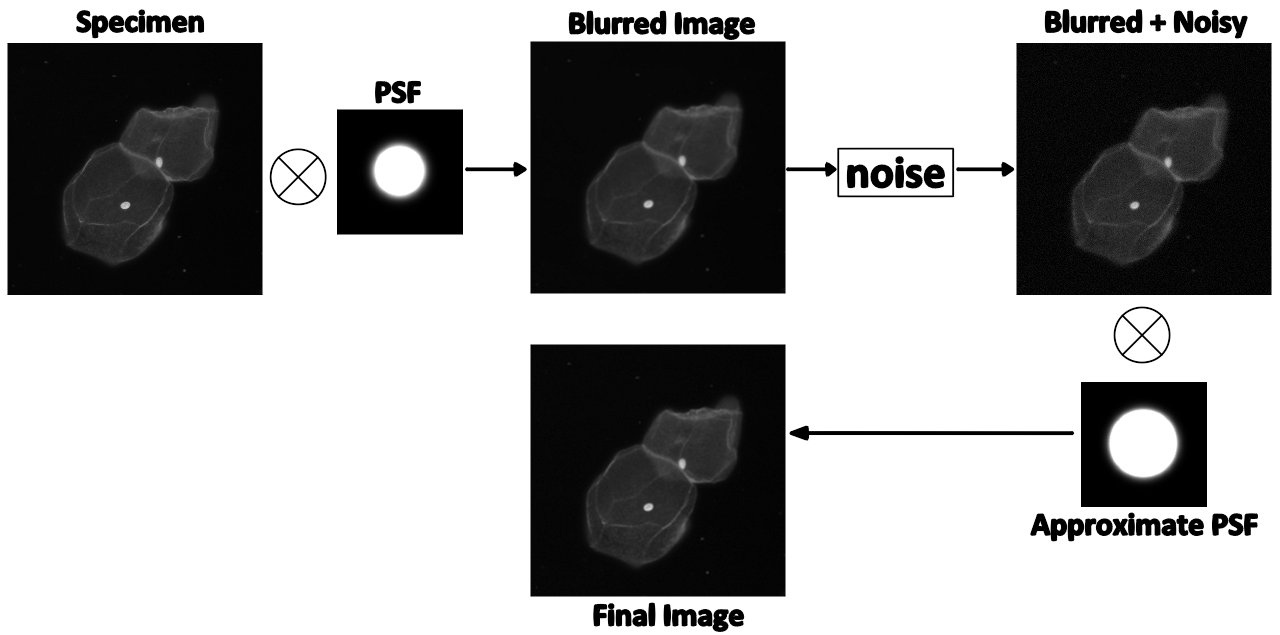
\includegraphics[width=\columnwidth]{image_formation.png}
		\caption{The image formation process. Image source: \citep{cil:40968}}
		\label{fig:imageformation}
	\end{figure}
	
	%Image deconvolution is a well researched and still an ongoing research topic.
	Deconvolution has recieved a lot of attention in the passed with very creative approaches \citep{Mukamel2012,Verveer2007,Periasamy1999,Swedlow2007,Rooi2014}.
	Fluorescence microscopy deconvolution is still a very active field of research.
	Bayesian methods have become popular in fluorescence microscopy image deconvolution, however noise in low SNR imaging conditions still poses a challenge \citep{Wong2015}.
	Recent trends in 3D deconvolution in widefield microscopy use blind depth-invariant of the PSF \citep{Kim2015}.
	Most PSF deconvolution systems na{\"i}vely assume depth-invariance however, the PSF changes significantly along the optical axis.
	There are also deconvolution methods that can preserve detail and possibly enhance image quality in diffraction-limited/superresolution imaging modalilities \citep{Qin2016}.
\end{definition}

\begin{definition}[Noise]
\textcolor{red}{What types of noise are most prevalent? How do they arise? What techniques are done to reduce it's effect.}
As previously stated, fluorescence imaging is a low light, low constrast and low SNR imaging technique to counter the effects of bleaching.
For these reasons, noise becomes prominent. The three types of noise recorded by a camera is \textit{dark noise}, \textit{read noise} and \textit{photon noise} \citep{Dobrucki2013,Danek2012,Matula2012,Hubeny2008}.

The electrons in a CCD of film are always in motion due to thermal energy.
Dark current is due to the extraneous electrons which excited into the signal.
This signal carries a statistical fluctuation known as dark noise.
Dark current effects can be reduced by ground image subtraction or cooling the CCD.
If there is a significant amount of dark noise then the background won't be as black as it should be.
For this reason it is common to mistake dark noise for low-level autofluorescence \citep{Ryan2016,Dobrucki2013}.

Read noise is a result of the conversion process from charge build-up to a voltage and then digitisation.

Photon noise, also known as \textit{shot noise}, is the signal dependant statical variation of the counting of photons incident on the CCD or film.
This is a naturally occuring phenomenon and cannot be reduced by camera design of system optimisation \cite{Ryan2016}.

In low-light imaging techniques, such as is common in fluorescence imaging, the dominant form of noise is photon noise.
Photon noise and dark noise are Poisson distributed \citep{Danek2012,Ryan2016,Kempen1999}.
Noise is low-light images used to modelled using the Gaussian distribution but was found to be a poor description of the noise.
The Poisson distribution provides a more physically accurate model especially in photon-limited recording \citep{Sarder2006}.
We study deonising in \Cref{sec:PoissonDenoising}.
The effect of noise on segementation accuracy is illustrated in \autoref{fig:Noise}.

\begin{figure}[!t]
	\centering
	\subfigure[]
	{
		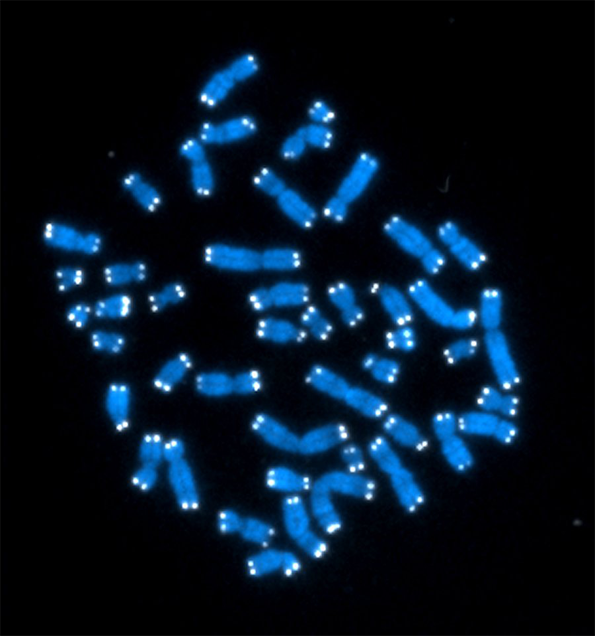
\includegraphics[width=0.31\columnwidth]{poisson2.png}
		\label{fig:ImageProcessingOriginal3}
	}
	\subfigure[]
	{
		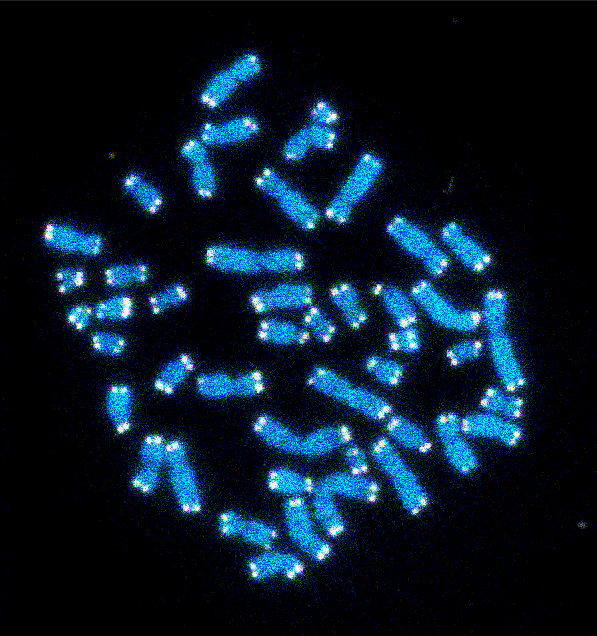
\includegraphics[width=0.31\columnwidth]{poisson.png}
		\label{fig:PoissonNoise}
	}
	\subfigure[]
	{
		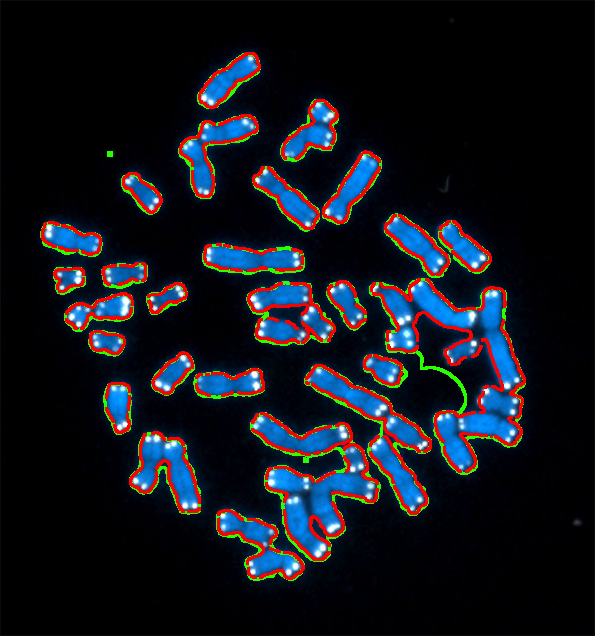
\includegraphics[width=0.31\columnwidth]{poisson_final.png}
		\label{fig:NoiseSegmented}
	}
	\caption{The effect of noise on segmentation. 
		\textbf{(a)} Original image. 
		\textbf{(b)} Poisson noise corrupted image.
		\textbf{(c)} ACWE Chan-Vese segmentated output. The red curve is from the original, the green curve is from the Poisson noise corrupted image. Notice that there are more artifacts and the segmented output is less accurate especially towards the bottom left from the green curve.}
	\label{fig:Noise}
\end{figure}
\end{definition}

\subsection{Segmentation}
\textcolor{red}{Write a little something on segmentation in cell imaging. Basic historical track of cell segmentation. Focus on specfic segmentation techniques.}
The primary aim of using fluorescence microscopy imaging is to make diagnoses and to study molecular behaviour and interaction.
This means that biologists, geneticists and other professionals alike, not only have a superabundance of microscopic imaging techniques at their disposal, but also have an immense amount of image data to analyse since the outburst of image acquisition technology.
The abundance, diversity, dimensionality and complexity of fluorescence image data obviates manual image processing as this isn't tractable, by any means, in terms of time or quality \citep{Meijering2012,Ryan2016}.
Consequently, the task has fallen to computers to perform these tasks and has now become of essential in advancing these fields \citep{Alberts2007,Vonesch2006}.
The crux of image analysis lies on the accuracy of image segmentation and has become the principle focus in many studies \citep{Bengtsson2004}.\\

Anton van Leeuwenhoek, a Dutch draper and scientist, is credited with the invention of the first real compound microscope in the late 17th century.
However, it wasn't until the mid-1950s that computers became involved when systems were developed to automate the classification of smears of exfoliated cells.
These systems used simple thresholding rules on 1D scanning of microscopic lines \citep{Tolles1955}.
In the 1960s, automated systems were developed to count leukocytes on 2D image data based on their colour and morphological measurements \citep{Prewitt1966}.
In the 1980s the invention of the confocal microscope made it possible to study cells in 3D but it wasn't until the 1990s that computer became powerful enough to process 3D image data or complex 2D images \citep{Gurcan2009}.
The trends of increased computing power has made possible the use of more sophisticated cell analysis techniques as well as the ability to use more computationally demanding segmentation methods.
The literature on cell segmentation and analysis has experienced exponential growth in the last couple of decades.
Many studies comparing segmentation algorithms for cells have been pubished \citep{Dima2011,Pincus2007,Coelho2009}.
We review some of the common techniques used in fluorescence microscopy image segmentation.

\begin{definition}[Intensity thresholding]
	\textcolor{red}{Say something about this section.}
	Intensity thresholding assumes a non-overlapping intensity levels between the objects and the background.
	It is still one of the most common thresholding methods for cell segmentation \citep{WuMerchantCastleman2008,Meijering2004,Quanli2011}.
	Locally adaptive thresholding techniques are used when illumination varies across the image.
	Automated threshold segmentation techniques are usually based on global or local intensity using the histogram \citep{Bengtsson2004}.
	Thresholding produces suboptimal results due to the na{\"i}ve assumption of mutually exclusive intensity levels.
\end{definition}

\begin{definition}[Morphological segmentation]
	\textcolor{red}{Say something about this section.}
	This method uses non-linear mathematical morphological operators like erosion, dilation, opening, closing, etc with geometrical and topological properties to segment the image \citep{GonzalezWoods2002,Meijering2004,Dorini2007,Anoraganingrum1999,Kumar2002}.
	Generally, this method is used as a post-processing step to polish up coarse segmentation or a pre-processing step to suppress certain image structures \citep{Bengtsson2004}.
\end{definition}

\begin{definition}[Region accumulation]
	\textcolor{red}{Say something about this section.}
	This method starts with selected points, called seeds.
	The idea is to iteratively add points neighboring previously labelled pixels based on some conformity measure, usually intensity.
	The most common implementation is called \textit{region growing}.
	Most cases assume an image model similar to that of thresholding and suffers the same segmented results problems.
	Another approach is called the \textit{watershed method} which converts the image into an open 3D shape and "fills the shape with water".
	The different regions are separated by those "filled with water" and those that aren't.
	A common problem with this method is oversegmentation and usually requires post-processing methods, like \textit{region merging}, to get a meaningful result \citep{Jiang2003,Lin2003,Bengtsson2004}.
\end{definition}

\begin{definition}[Edge-based segmentation]
	\textcolor{red}{Say something about this section.}
	There are basically two types of edge-based segmentation: \textit{gradient based methods} and \textit{Laplacian based methods}.
	
	Gradient methods are based on the assumption that there is a rapid intensity gradient between the object and the background.
	Edges are detected by searching for the maximum and minimum in the first derivative, e.g. Prewitt, Roberts and Sobel operators.
	
	Laplacian methods search for zero-crossings in the second derivative, e.g. Marr-Hildreth, Laplacian of Gaussian (LoG), Canny edge detection.
	
	These algorithms are very fast to compute but the drawback is when closed curves are desired \citep{Bengtsson2004}, which is a common criterion in biological and molecular segmentation.
	A solution to this is to use snakes or active shape models.
\end{definition}

\begin{definition}[Energy minimisation]
	\textcolor{red}{Two types: Deformable models and Graph cuts}
	The most recent segmentation methods are based on energy minimisation.
	Most current state-of-the-art techniques fall under this category.
	This is due to their flexibility and robustness \citep{Danek2012}.
	This group encompasses two main subgroups: \textit{deformable models} and \textit{discrete combinatorial optimisation}.
	
	The aim of deformable model techniques is to fit a deformable model, either a curve or a surface, to the image data.
	They may be formulated either explicitely, as a parametric contour (2D) or a surface, e.g. snakes \citep{Kass1988} or active contours \citep{Caselles1997,Li2009,Cheng2009}, or implicitely as a zero-level of a function with one dimension higher than that of the image data, e.g. as a level set \citep{Osher2003}.
	This technique widely used in fluorescence image segmentation \citep{Dzyubachyk2008,Ortiz2001,Dufour2005,Dzyubachyk2010,Boukari2014,Maska2007}.
	
	The aim discrete combinatorial optimisation is to search a finite countable solution space for the optimal solution.
	Optimality is defined with respect to some energy function, which embeds one or more criteria, which is to be minimised.
	The most common implementation exploits the graph cut framework.
	Graph cut segmentation has recently gained a lot of popularity and momentum in medical image segmentation (MIS) \citep{Danek2009,Chen2008,Kofahi2010,Kong2011,Yang2009,Zhang2014,Liu2008,Vu2008}.
\end{definition}

\begin{definition}[Other miscellaneous techniques]
	\textcolor{red}{Unsupervised clustering (k-means), Otsu binarization , dynamic programming , Voronoi diagrams , ellipse fitting, template matching, model matching, gradient flow tracking.}
	The techniques presented are just a select few in a plethora segmentation techniques that have been used in microscopy image segmentation.
	A few other common techniques are unsupervised clustering segmentation using the k-means \citep{Ng2006,Shrivastava2014,Dhanachandra2015}, Otsu binarization \citep{Chen2006}, dynamic programming \citep{Liu2007,Zhang2007}, Voronoi diagrams \citep{Cardenes2003,Jiang2005}, gradient flow tracking \citep{Li2007}, etc.
	This is just a few more.
	Instead of cell segmentation converging to a robust, flexible and unified solution, the number of available options is steadily increasing \citep{Meijering2012}.
	There probably exists as many individual unique solutions for cell segmentation as there are problems.
\end{definition}

%----------------------------------------------------------------------------------------
%	SECTION 5
%----------------------------------------------------------------------------------------

\section{Object Measurement and Analysis}
\label{sec:Measurements}

\textcolor{red}{What is the purpose of object analysis in FM? What is measured?}
The aim in fluorescence image analysis is to measure specific properties of interest which enable higher level decision making.
Typically, these properties are quantitative measures.
In this section we review some of the important quantitative measurements in digital image analysis.
It is important to note that for some of the properties of interest, the accuracy of the measurements depend heavily on the accuracy on the segmentation.
The properties of interest are application dependent, one might require just the object morphology of structure and hence properties like perimeter, area, shape, intensity, colour, etc are of significance.
Alternatively, if one requires the colocalisation of cells, then distance discriminants, such as Euclidean distance, Manhattan distance, Chessboard distance, etc, are of significance \citep{Fatima2008_2,Danek2012}.

Object measures can be loosely classified into four catergories: geometric measures, histogram-based measures, intensity based measures and temporal measures. One can also argue a fifth catergory statistical classifiers although this is generally used in higher level analysis.

\begin{definition}[Size measures]
	Perimeter, area and volume are common measures to describe the size of objects.
	Area and volume are suitable measures to describe the general size of an object.
	The perimeter of an object is distinctly useful in discriminating its shape complexity. Complex and irregular shapes need a larger perimeter to enclose its area.
\end{definition}

\begin{definition}[Pose measures]
	This measure is defines an objects location and orientation.
	The centroid is used as an objects' locale and its orientation is the measure of the angle subtended by its major axis.
\end{definition}

\begin{definition}[Shape measures]
	Shape features are used to distinguish objects from one another.
	These measures are generally translationally, rotationally and scale invariant and can be used independent of, or in conjunction with, the size measures.
	Commonly assessed shape parameters are thinness ratio to describe the regularity of an object, rectangularity, circularity, Euler number, moments, central moments, object dispersion, rotationally invariant moments, Zernike moments and elongation.
\end{definition}

\begin{definition}[Shape descriptors]
	Shapes descriptors provide a more wholesome way of decribing an object's shape than compared to the single parameter shape measures.
	Differential chain codes, and its two most common descriptors boundary chain code (BCC) and differential chain code (DCC), are used to represent the distance around an object.
	Fourier descriptors is another object distance measure that expliots the periodicity of BCC.
	There are also graph respresentations of which the two most common are minimum spanning tree (MST) \citep{Giesen2014,Yuan2009} and Delaunay triagulation (DT) \citep{Kozubek2000,Attali1997}.
\end{definition}

\begin{definition}[Distance measures]
	There are many ways to compute the separation between objects.
	The most commonly assessed distance measures are Euclidean distance, Manhattan distance (also known as the City-block distance or absolute value metric), which is a more computationally efficient approximation of Euclidean distance, and the Chessboard distance (also known as the maximum value metric) \citep{French2008,Zinchuk2007}.
\end{definition}

\begin{definition}[Intensity measures]
	Images are segmented generally into region with low intra-region intensity distribution and high inter-region intensity distribution \citep{Pinkel1986,Meijering2004}.
	Common intensity measures are integrated optical density (IOD) \citep{Loferer1998,Watanabe1991}, is simply the sum of all the gray levels that compose the object, its a reflection of  the object's "mass" or "weight", average optical density (AOD), is the IOD divided by the objects area, and contrast.
\end{definition}

\begin{definition}[Histogram measures]
	These measure provide a measure of an object's intensity distribution.
	Common histogram-based measures are mean, standard deviation, skew, entropy and energy \citep{Rust2006,Boland2001}.
\end{definition}

\begin{definition}[Texture measures]
	In image analysis texture refers to the spatial arrangement of gray level values \citep{Duda2001} and hence a texture feature quantifies some characteristic of the intensity variation within an object.
	Common texture measures are statistical texture measures, gray-level co-occurrence matrix (GLCM) \citep{Atlamazoglou2001,Cicchi2010} and power spectrum features \citep{Erik1999,Xu1996}.
\end{definition}

\begin{definition}[Ratiometric measures]
	Some fluorescent dye respond to the changes in Calcium and Hydrogen ion concentration by changing its spectral properties of the fluorescent emission bands. In this case, a ratio of the intensity can be used to calculate concentration of calcium of pH value \citep{Dobrucki2013}.
\end{definition}

\begin{definition}[Temporal measures]
	Considering the time domain, many interesting properties can be observed.
	Commonly computed properties of interest are motility \citep{Sekar2003,Miller1869,Mathur2000}, like velocity and acceleration, rate of growth, rate of change of colour, etc.
\end{definition}

These measures are used in higher decision making processes such as the evaluation of a hypothesis to detect the presence of a certain disease. They are also used to aid in the understanding of biological mechanisms, events and interatctions \citep{Danek2012}.